\documentclass[crop,tikz,pgf]{standalone}

\usetikzlibrary{arrows,automata,positioning}

\begin{document}
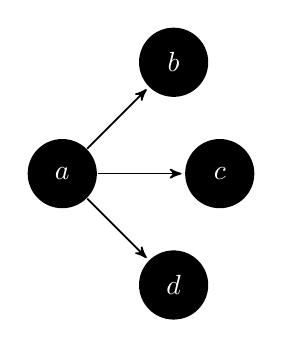
\begin{tikzpicture}[->,>=stealth',shorten >=1pt,auto,node distance=2cm,semithick]
	\tikzstyle{every state}=[fill=black,draw=none,text=white]

	\node[state] (A) {$a$};
	\node[state] (B) [above right of = A] {$b$};
	\node[state] (C) [right of = A] {$c$};
	\node[state] (D) [below right of = A] {$d$};

	\path (A) edge (B);
        \path (A) edge (C);
        \path (A) edge (D);
\end{tikzpicture}
\end{document}